\subsection{Erdvės diskretizavimas Dekarto koordinačių sistemoje}

Dviejų dimensijų skaitiniam modeliui erdvė buvo padalinta į $N \times M$ taškų 
nutolusių vienas nuo kito fiksuotais $\Delta x$ ir $\Delta y$ atstumais.

\begin{figure}[!h]
\centering
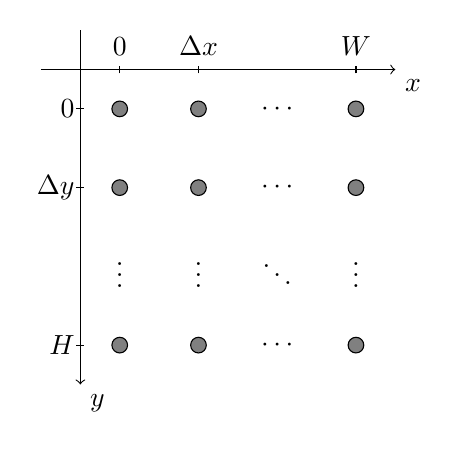
\begin{tikzpicture}

   % Set up styles for the grid
  \tikzset{
    node/.style={circle, draw, fill=gray, inner sep=2pt},
    ellipsis/.style={draw=none, fill=none}
  }

  \draw[->] (0, -0.5) -- (4.5, -0.5) node[anchor=north west] {$x$};  % x-axis
  % x-axis ticks
  \draw[-] (1, -0.55) -- (1, -0.45) node[anchor=south] {$0$};
  \draw[-] (2, -0.55) -- (2, -0.45) node[anchor=south] {$\Delta x$};
  \draw[-] (4, -0.55) -- (4, -0.45) node[anchor=south] {$W$};
  
  \draw[<-] (0.5,-4.5) node[anchor=north west] {$y$} -- (0.5, 0);  % y-axis
  % y-axis ticks
  \draw[-] (0.45, -1) -- (0.55, -1) node[anchor=east] {$0$};
  \draw[-] (0.45, -2) -- (0.55, -2) node[anchor=east] {$\Delta y$};
  \draw[-] (0.45, -4) -- (0.55, -4) node[anchor=east] {$H$};


  % Draw the 3x3 grid of colored circles in a 4x4 layout
  \foreach \x in {1, 2, 4} {
    \foreach \y in {1, 2, 4} {
      \node[node] at (\x, -\y) {};
    }
  }

  % Add ellipses in the 4th row and column for continuation

  \node[ellipsis] at (3, -1) {$\cdots$};
  \node[ellipsis] at (3, -2) {$\cdots$};
  \node[ellipsis] at (3, -4) {$\cdots$};

  \node[ellipsis] at (1, -3) {$\vdots$};
  \node[ellipsis] at (2, -3) {$\vdots$};
  \node[ellipsis] at (4, -3) {$\vdots$};

  \node[ellipsis] at (3, -3) {$\ddots$};

\end{tikzpicture}
\caption{ diskretizuota erdvė }
\end{figure}

Čia 